% The MIT License (MIT)
% 
% Copyright (c) 2013, Gergely Nagy
% 
% Permission is hereby granted, free of charge, to any person obtaining a copy
% of this software and associated documentation files (the "Software"), to deal
% in the Software without restriction, including without limitation the rights
% to use, copy, modify, merge, publish, distribute, sublicense, and/or sell
% copies of the Software, and to permit persons to whom the Software is
% furnished to do so, subject to the following conditions:
% 
% The above copyright notice and this permission notice shall be included in
% all copies or substantial portions of the Software.
% 
% THE SOFTWARE IS PROVIDED "AS IS", WITHOUT WARRANTY OF ANY KIND, EXPRESS OR
% IMPLIED, INCLUDING BUT NOT LIMITED TO THE WARRANTIES OF MERCHANTABILITY,
% FITNESS FOR A PARTICULAR PURPOSE AND NONINFRINGEMENT. IN NO EVENT SHALL THE
% AUTHORS OR COPYRIGHT HOLDERS BE LIABLE FOR ANY CLAIM, DAMAGES OR OTHER
% LIABILITY, WHETHER IN AN ACTION OF CONTRACT, TORT OR OTHERWISE, ARISING FROM,
% OUT OF OR IN CONNECTION WITH THE SOFTWARE OR THE USE OR OTHER DEALINGS IN
% THE SOFTWARE.
\documentclass[12pt]{article}
\usepackage[paper=a4paper, margin=2.5cm]{geometry}
\usepackage{fancyhdr}
\usepackage[utf8]{inputenc}
\usepackage[english]{babel}
\usepackage[pdfborder={0 0 0}]{hyperref}
\usepackage{setspace}
\usepackage[T1]{fontenc}
\usepackage[lighttt]{lmodern}	%needed to have bold teletype (to have bold keywords in lstlisting)
\usepackage{hfoldsty}			%has to go after \usepackage{lmodern} to take effect
\usepackage{listings}
\usepackage{graphicx}

\pagestyle{fancy}
\fancyhf{}
\renewcommand{\headrulewidth}{0pt}
\renewcommand{\footrulewidth}{0pt}
\fancyhf[FL]{\scriptsize{\textit{The SyntX Parser Library (Gergely Nagy)}}}
\fancyhf[FC]{\scriptsize{\textit{\textbf{\thepage}}}}
\fancyhf[FR]{\scriptsize{\textit{\today}}}

%\lstset{basicstyle=\scriptsize\ttfamily, keywordstyle=\bfseries\ttfamily}
\lstset{basicstyle=\scriptsize\ttfamily, stringstyle=\ttfamily,
keywordstyle=\bfseries\ttfamily,aboveskip=10pt,
belowskip=10pt, tabsize=2, xleftmargin=5pt, captionpos=b, 
literate={á}{{\'a}}1 {é}{{\'e}}1 {ó}{{\'o}}1 {ö}{{\"o}}1 {ú}{{\'u}}1 {ü}{{\"u}}1}

\newcommand{\usec}[2]{\section*{#1}\label{sec:#2}\addcontentsline{toc}{section}{#1}}
\newcommand{\usubsec}[2]{\subsection*{#1}\label{subsec:#2}\addcontentsline{toc}{subsection}{#1}}

\begin{document}
\sloppy

\vspace*{2em}
\centerline{\Huge\textbf{The SyntX Parser Library}}
\vspace{5em}

\begin{center}
	\begin{minipage}[h]{0.85\linewidth}
		\itshape
		The SyntX parser library is a set of C++ classes that enables users to create a parser for an LL(k)
		grammar by giving the production rules with an EBNF-like notation in the form of C++ expressions.
		There is thus no need for a precompiler, the parser can be an integral part of a C++ project.
	\end{minipage}
\end{center}

\vspace{4.5em}

\usec{Recursive descent parsing}{rdp}
The SyntX library is based upon the theory of recursive descent parsers (RDPs). In order to gain a deep and confident
understanding of the library, one has to be familiar with the fundamentals of recursive descent parsing.

This section provides a brief introduction with a very simple example. It also introduces some of the types
and notations that are used in the source code of the library as well.

\usubsec{The Extended Backus-Naur Form}{ebnf}
EBNF\footnote{Extended Backus-Naur Form --
\href{http://en.wikipedia.org/wiki/Ebnf}{en.wikipedia.org/wiki/Ebnf}} is a widespread notation that can be
used to express context-free grammars. It is the extension of the Backus-Naur Form (BNF). Actually several
EBNF styles exist -- this document uses the one defined by W3C\footnote{World Wide Web Consortium --
\href{http://www.w3.org}{www.w3.org}}.

The "Hello World" grammar that is generally used to introduce parsing describes a mathematical expression
containg numbers, the four basic operations and an arbitrary depth of parentheses. The grammar below is even
simpler than that, it allows only addition, so the way precedence can be handled is not shown. It allows an
infinite depth of grouping using parentheses however. The ease with which recursive structures can be handled
by EBNF grammars and RDPs is a very important feature and is often exploited.

\begin{center}
	\begin{minipage}[h]{0.5\textwidth}\label{lst:hellogrammar}
		\begin{lstlisting}[breaklines=true]
addition = addend ('+' addend)*
addend = [0-9] | expression
expression = '(' addition ')'
		\end{lstlisting}
	\end{minipage}
\end{center}

The production rule named \texttt{addition} is the \emph{start rule}. The text that we're trying to analyze
should conform to this rule as a whole. The details can be investigated by following the references to other
rules.

The \texttt{addition} rule states that an addition is made up of an addend that can be followed by an
arbitrary number of addends each preceded by a '+' operator. The \texttt{*} operator in EBNF allows zero or
more occurence of a match (or a sequence of matches). This means that an addition may consist of a single
addend as well, which is OK: a number can be thought of as a mathematical expression.

If we wanted to have at least two addends seperated by a '+' operator, than EBNF's operator \texttt{+} should
be used, which allows one or more occurences.

An addend in our simple grammar can be either a single digit (given here by the shorthand used to describe
character sequences in EBNF) or an expression. The \texttt{|} operator stands for \emph{alternation}.

The interesting part lies in the \texttt{expression} rule. An expression is an addition enclosed by
parantheses. This is how the grammar becomes recursive and how an expression of infinite complexity can be
described by a handful of production rules.

Let's see some examples! The simplest possible expression is a single digit:

\begin{center}
	\begin{minipage}[h]{0.1\textwidth}
		\begin{lstlisting}[breaklines=true]
8
		\end{lstlisting}
	\end{minipage}
\end{center}

The start rule is where the matching starts, so we assume that the our text is an \texttt{addition}. An addition starts
with an \texttt{addend}. An \texttt{addend} can be a digit so the text indeed starts with an addend. Thus the
first part of the \texttt{addition} rule matched, we may move on to the rest of the text. Next we're looking
for a '+' character which we don't find. Luckily this part of the rule is optional, so we get to the end of
the rule having matched the entire text. This is a successful match.

Let's go for something more complex next:

\begin{center}
	\begin{minipage}[h]{0.2\textwidth}
		\begin{lstlisting}[breaklines=true]
2 + 3 + (4 + 8)
		\end{lstlisting}
	\end{minipage}
\end{center}

The \texttt{addition} rule will find two digits with a '+' character in between. It could already stop there
as we have a sum which complies to the rules, but we haven't reached the end of the text and actually the
rule allows more than two addends. So the parsing continues, we find a second '+' character and then an
opening parenthesis. This is OK, as the \texttt{addend} rule doesn't only match digits, \texttt{expression}s
are also allowed.

So next we're trying to match the \texttt{expression} rule which contains an \texttt{addition} between
parentheses. That's exactly what we have here so, again, we have a successful match. Please note that the
\texttt{addition} inside the \texttt{expression} can again turn into an \texttt{expression} and then into an
\texttt{addition} -- this is exactly how the arbitrary depth of the expression is analyzed.

\usubsec{Functions corresponding to each production rule}{parsingfun}
One way to realize a recursive descent parser in a programming language is to create a function corresponding
to every production rule. These functions receive the context of parsing (i.e. the text to be parsed and the
current position) and return a Boolean value which is true if the function could match a certain substring of
the text and could move the position further towards the end of the text. If the function returns false, the
position is not altered.

Following is an example function that matches one character of the text if it can be found in the string
serving as a character set taken as an argument. The structure of this function is characteristic of the
rule methods in the SyntX library.

\begin{center}
	\begin{minipage}[h]{0.8\textwidth}\label{lst:globalcharacter}
		\begin{lstlisting}[language=C++, breaklines=true, numbers=left]
bool character(match_range &context, std::string const &characters) {
  match_range local = context;

  if (local.first == local.second) return false;

  for (auto c: characters) {
    if (*local.first == c) {
      ++local.first;
      context.first = local.first;
      return true;
    }
  }

  return false;
}
		\end{lstlisting}
	\end{minipage}
\end{center}

The \texttt{match\_range} type is an \texttt{std::pair} that holds two \texttt{string::const\_iterator}s. It
describes the context of the parsing: the first element points to the current position (the character that
should be analyzed next), the second to the end of the text.

\begin{center}
	\begin{minipage}[h]{0.8\textwidth}\label{lst:matchrange}
		\begin{lstlisting}[language=C++, breaklines=true]
using match_range = std::pair< std::string::const_iterator,
                               std::string::const_iterator >;
		\end{lstlisting}
	\end{minipage}
\end{center}

The function has two arguments, the context and the character set that contains the characters that are
accepted. The context is taken as a non-constant reference because the function sets the current position
after the the last character it could match.

In line~2 a copy of the context is created. This copy will reflect the analysis performed by the function. A
complex parser function can delve deep into a string before finding out that it doesn't match it after all. It
might also call a series of other parsing functions on the way that also alter this value, so it is absolutely
necessary to keep a copy of the original position and only change that value when there is a successful match.

Every parser function that operates at the character level should always check whether the end of the text has
been reached. This can be seen in line~4.

As long as a function finds characters it can consume, it advances the current position, i.e. the first
element in the local copy of the context (line~8).

If a function matches a certain substring of the text and cannot advance further, two things need to be done:
the context taken by reference has to be changed to reflect the advancement in the analysis of the text and it
has to return \texttt{true} (lines~9-10). Otherwise it has to merely return \texttt{false} (line~14), the
context is left unchanged.

\usubsec{Recursive descent}{recdesc}
The example above shows a simple parsing function working at the character level. It doesn't call any other
function, instead it decides on its own whether the text at the given position matches it or not. This is
because that rule describes a so called \emph{terminal symbol}, one that corresponds to a symbol actually
appearing in the text, in this case, a letter.

Other rules might define symbols that contain other symbols and define a structure that these symbols should
have in order to comply to the rule. The composite symbols are called \emph{non-terminal symbols}.

In RDPs non-terminal symbols can be parsed using functions that call other parsing functions just as any rule
can be referenced in the definition of an EBNF rule.

Let's see an example for such a function: the \texttt{expression} rule in the simple grammar seen earlier.

\begin{center}
	\begin{minipage}[h]{0.8\textwidth}
		\begin{lstlisting}[language=C++, breaklines=true, numbers=left]
bool expression(match_range &context) {
	match_range local = context;

	if  (
		character(local, "(") && addition(local) && character(local, ")")
	) {
		context.first = local.first;
		return true;
	}

	return false;
}
		\end{lstlisting}
	\end{minipage}
\end{center}

It is interesting to note that as this function doesn't operate at the character level (every character
consumed by the rule is processed by one of the functions called by it), it doesn't need to check for the end
of the text -- it has to be done by the low-level functions.

The sequence of the sub-rules is realized by the \texttt{\&\&} operator of the C++ language. Short-circuit
evaluation is exploited here: if the first rule doesn't match and thus returns \texttt{false} then the second
is not called and the entire expression will evaluate to \texttt{false}.

Furthermore, the order of evaluation is fixed too and goes from the left to the right. So \texttt{addition}
will receive an updated \texttt{local} -- the value that was altered by the first call to \texttt{character}.

So, when all three functions return \texttt{true}, the body of the \texttt{if} statement is evaluated and
\texttt{context} receives a value updated by all three functions and now pointing to the next position of the
text to be parsed.

Alternatives can be realized using the \texttt{||} operator where short-circuit evaluation comes handy again
as the second function gets called only if the first failed to match (in which case the first doesn't alter
the context which is also important).

Please note that composite logical expressions should not be constructed as they can lead to mispositioned
iterators. Let's investigate the following code fragment:

\begin{center}
	\begin{minipage}[h]{0.8\textwidth}
		\begin{lstlisting}[language=C++, breaklines=true, numbers=left]
if (
	(rule1(local) && rule2(local)) || rule3(local)
) {
	...
}
		\end{lstlisting}
	\end{minipage}
\end{center}

Let's assume that \texttt{rule1} matches but \texttt{rule2} doesn't, so \texttt{rule3} gets a chance. The
problem is that \texttt{rule1} moves the position that \texttt{local} points to. Unfortunately it doesn't get
corrected before \texttt{local} is fed to \texttt{rule3} so \texttt{rule3} will try to match from a different
position then the one where \texttt{rule1} started from and this is not what we intended to do.

If the above expression is realized in two seperate functions, one containing the sequence (AND logic) and the
other containing the option (OR logic) then this situation doesn't occur as the functions will only alter the
context if they match. This is done automatically in the SyntX framework but it is something the programmer
has to pay attention to if the parser is handwritten.

\usubsec{Actions during parsing}{actions}
All the example functions shown up to here did was to tell whether their input complied to their requirements
or not. If the task of the parser is merely to determine if a text conforms to a specific grammar then this is
sufficient. Otherwise the functions should perform operations to yield a result of the parsing. This can be in
the form of an AST (abstract syntax tree) or pratically any data that can be generated based on the input.

When the parsing functions are handwritten the actions to be performed when a match is found can be put inside
the parsing function resulting in a code where parsing and data processing is intertwined. For simple problems
this is a perfect solution and is easy to handle.

When problems become more complex this method becomes tiresome or even impracticable: there are cases where
data processing cannot be performed at the time of parsing as additional knowledge is needed that can only be
extracted later, possibly after the parsing of the entire input is finished.

In the SyntX framework a \texttt{std::function} (which can wrap a plain function, a method, a function object
or a lambda) can be assigned to any rule -- these are called \emph{action}s. The function receives the matched
range as a \texttt{std::string} and can do whatever is needed when the given rule is successfully matched.

There is just one problem with this approach: if a complex data is defined by a sequence of rules such as in
this case

\begin{center}
	\begin{minipage}[h]{0.8\textwidth}
		\begin{lstlisting}[breaklines=true]
complex = rule1 rule2 rule3
		\end{lstlisting}
	\end{minipage}
\end{center}

\noindent then we cannot be sure that the entire expression will match until \texttt{rule3} returns
\texttt{true}. The problem is that we need to extract the results on a rule-basis, otherwise we get the
matched range of the three rules packed in one string needing yet another extraction.

A solution to this problem can be to store the results of the three rules in temporary variables and build the
complex data only when all three matched successfully.

In SyntX actions are added to rules using \texttt{operator[]} and they can be assigned to a group of rules as
well:

\begin{center}
	\begin{minipage}[h]{0.8\textwidth}
		\begin{lstlisting}[breaklines=true]
complex = ( rule1[action1] rule2[action2] rule3[action3] )[action4]
		\end{lstlisting}
	\end{minipage}
\end{center}

Actions~1-3 should place the results of the matches in temporary variables and action~4 should construct the
complex data.

Please note that this is not exactly the correct syntax -- it is only shown for demonstration purposes here.

\usec{The SyntX framework}{syntx}
In the next few subsections the framework's structure and the basics of its operation are explained briefly. For
the details please refer to the Doxygen documentation, which can be generated from the source code with the
help of the Makefile provided with the project (\texttt{make docs}).

\usubsec{The \texttt{base\_rule} class}{baserule}
The base class of every rule is \texttt{base\_rule}. It defines two data types used throughout the framework,
contains the semantic action assigned to a rule and performs the basic administrative tasks concerning the
matching process. The exact instructions regarding the matching have to go in a virtual function defined as
pure virtual in this class (\texttt{test}).

One of the data types define in \texttt{base\_rule} has already been mentioned on page
\pageref{lst:matchrange}, it is the \texttt{match\_range} which is used for two purposes: it defines the
limits between which the parsing is done and also the range matched by a given rule.

The other type is \texttt{semantic\_action} discussed earlier on page \pageref{subsec:actions}:

\begin{center}
	\begin{minipage}[h]{0.8\textwidth}
		\begin{lstlisting}[language=C++, breaklines=true]
using semantic_action = std::function<void(std::string const &)>;
		\end{lstlisting}
	\end{minipage}
\end{center}

One action can be assigned to a rule and it's stored in the \texttt{the\_semantic\_action} data member of the
class.

The \texttt{match} method handles the tasks associated with matching\footnote{This is not the actual code of
the function -- the parts concerning the automatic AST generation are discussed on page \pageref{subsec:ast}.
This is true for the coming examples as well.}.

\begin{center}
	\begin{minipage}[h]{0.8\textwidth}
		\begin{lstlisting}[language=C++, breaklines=true, numbers=left]
bool base_rule::match(match_range &context, match_range &the_match_range) {
	match_range a_range;

	if (test(context, a_range)) {
		the_match_range = a_range;

		if (the_semantic_action) {
			std::string the_matched_substring(the_match_range.first, the_match_range.second);
			the_semantic_action(the_matched_substring);
		}

		return true;
	}
	else return false;
}
		\end{lstlisting}
	\end{minipage}
\end{center}

The \texttt{match} method calls the virtual \texttt{test} to find out whether the text conforms to the rule at
the current position. If it doesn't, the method simply returns \texttt{false}, while in the case of a
successful match, the matched range is stored in the local variable \texttt{a\_range}. This value is delegated
to \texttt{the\_match\_range}, which is a reference of a variable taken as an argument.

If a semantic action has been assigned to the rule, it is called and the result of the matching process is
given to it as a \texttt{std::string}.

The \texttt{base\_rule} class has a virtual funtion called \texttt{clone} the purpose of which is to make the
entire class hierarchy clonable. More on this can be found on page \pageref{subsec:rule}.

\usubsec{Example of a rule subclassed from \texttt{base\_rule}}{character}
Let's look at a simple example of how an actual rule can be created using the \texttt{base\_rule} class. It is
the realization of the previously discussed character rule (page \pageref{lst:globalcharacter}) in the SyntX
framework.

As the \texttt{test} function to be overridden has a fixed argument list, the set of allowed characters is given in
the constructor and stored as a data member. Only two functions need to be written: \texttt{clone} -- which is
basically a oneliner that dynamically creates a copy of the rule and \texttt{test}.

The code of \texttt{test} resembles closely the \texttt{character} function on page
\pageref{lst:globalcharacter}.

\begin{center}
	\begin{minipage}[h]{0.8\textwidth}
		\begin{lstlisting}[language=C++, breaklines=true, numbers=left]
bool character::test(base_rule::match_range &context, match_range &the_match_range) {
	if (context.first == context.second) return false;

	base_rule::match_range local_context = context;

	for (auto allowed_character: allowed_characters) {
		if (*local_context.first == allowed_character) {
			++local_context.first;

			the_match_range.first = context.first;
			the_match_range.second = local_context.first;
			context = local_context;
			return true;
		}
	}

	return false;
}
		\end{lstlisting}
	\end{minipage}
\end{center}

The same operations are performed as seen earlier. First the function checks whether the current parsing
position is at the end of the input or not. If the end has been reached there is nothing to do but return
\texttt{false}. This operation has to be done in every rule that operates at the character level.

If there is input to process a local copy of the context is created. This is not necessary in this case, in
fact this code shows the generic and recommended way of writing a rule.

Then it iterates over the set of allowed characters and if any of them matches the one at the current reading
position then the context is adjusted, the match range is set and \texttt{true} is returned.

The goal of this example was to show how easy it is to extend the framework with a new rule. In fact the
need to create new rules should arise very rarely as the framework contains a great number of simple classes
with which almost every task can be solved.

\usubsec{Realizing EBNF operators}{ebnfoperators}
Next we look at the realization of EBNF operators (sequence, alternation, etc.) as subclasses of
\texttt{base\_rule}. Naturally, these classes are never instantiated manually -- it would make the grammars
unreadable. There are operators that do this so that the grammars defined in SyntX will look very much like
their EBNF counterparts.

Our example is alternation which will try to match one of the two rules given to it. It will first try the
first one and then the second if the first fails. This means that the first rule will have a precedence over
the second and this should be kept in mind when constructing the grammar\footnote{This can be important when
the input matched by one of the rules is the starting substring of the one matched by the other. In such a
case, if the shorter rule comes first, it will match and the second will never be run. There could be a special
alternation rule which chooses the longer of the two matches, but SyntX doesn't provide such a rule -- it is easy to
write though.}.

The \texttt{alternation} class stores the \texttt{shared\_ptr}s of two rules and overrides \texttt{clone} and
\texttt{test}. Let's analyze the latter:

\begin{center}
	\begin{minipage}[h]{0.8\textwidth}
		\begin{lstlisting}[language=C++, breaklines=true, numbers=left]
bool alternation::test(base_rule::match_range &context, base_rule::match_range &the_match_range) {
	base_rule::match_range first_range, second_range;
	base_rule::match_range local_context = context;

	if (first->match(local_context, first_range)) {
		the_match_range = first_range;
		context = local_context;

		return true;
	}
	
	local_context = context;

	if (second->match(local_context, second_range)) {
		the_match_range = second_range;
		context = local_context;

		return true;
	}
	
	return false;
}
		\end{lstlisting}
	\end{minipage}
\end{center}

The function first tries to match the first rule. If it succeeds, \texttt{the\_match\_range} and
\texttt{context} is adjusted and \texttt{true} is returned.

If the first rule didn't match, then the local copy of the context is set to the original value and the second
rule is given a chance. Theoretically the \texttt{local\_context} should not be altered by the first rule if
it doesn't match, so line~12 is unnecessary -- it is there to make sure that no mistake is made even if the
first rule does not conform entirely to the expectations.

\usubsec{The \texttt{rule} class}{rule}
The operators that make the grammars EBNF-like also make the framework a bit complicated. Let's first consider
a single rule that contains only built-in rules such as the one in the following example (which doesn't follow
the correct syntax of the framework to ease the understanding):

\begin{center}
	\begin{minipage}[h]{0.8\textwidth}
		\begin{lstlisting}[breaklines=true]
binary_digit = (character("0") | character("1")) character("b")
		\end{lstlisting}
	\end{minipage}
\end{center}

In order to avoid memory leaks and to make grammars easier to write and read, the rules are not created
dinamically. This means that unnamed, temporary local variables are created on the right side of the
expression above (as e.g. \texttt{character("0")} is the constructor of the class \texttt{character}).

This means that \texttt{operator |}, which creates an \texttt{alternation}, receives two temporary objects as
arguments. As it needs to accept any kind of \texttt{base\_rule}s, it cannot take them by value, so the only
choice is to take them as constant reference. This is OK, as long as it doesn't want to store these values, as
the reference of temporaries should not be stored.

The problem is that every operator will indeed want to store the rules that are given to them -- as we have
seen that earlier on page \pageref{subsec:ebnfoperators}. This is because the evaluation of these expressions
happens long after their construction, so actually some kind of a syntax tree is built automatically, which is
traversed during the parsing process. Thus, the \texttt{test} method of the temporary rules is called long
after they get deleted.

The solution to this problem is to create copies of these rules. As it has been shown, not much is stored in
these rules (a few pointers and maybe short strings), so copying them is a relatively cheap operation.

The copies have to be made inside the operator functions that take the constant reference of the temporaries.
The problem here is that all they know of these rules is that they are subclasses of \texttt{base\_rule}.  The
\emph{virtual constructor idiom} comes handy in this situation, thus we need a \texttt{clone} function, a typical
solution used e.g. in heterogeneous containers in several languages. This is why \texttt{base\_rule} defines
the \texttt{clone} function as pure virtual -- it makes every subclass override it, so that the framework can
rely on its existence in every rule object.

And indeed, what e.g. \texttt{alternation} does in its constructor is that it instantly makes copies of the
two rules it receives using their \texttt{clone} function: 

\begin{center}
	\begin{minipage}[h]{0.8\textwidth}
		\begin{lstlisting}[language=C++, breaklines=true]
alternation::alternation(
	base_rule const &first,
	base_rule const &second
) : 
	first(first.clone()),
	second(second.clone()) {}
		\end{lstlisting}
	\end{minipage}
\end{center}

And all that \texttt{operator|} does is create an instance of \texttt{alternation} and returns it in a
\texttt{rule}:

\begin{center}
	\begin{minipage}[h]{0.8\textwidth}
		\begin{lstlisting}[language=C++, breaklines=true]
rule operator |(base_rule const &first, base_rule const &second) {
	return rule(
		std::shared_ptr<base_rule>(new alternation(first, second))
	);
}
		\end{lstlisting}
	\end{minipage}
\end{center}

We will soon get to why this is needed and what the purpose of class \texttt{rule} is.

If there were no rules that refer to other composite rules then we could stop here and there would be no need
for the \texttt{rule} class. We could build expressions of arbitrary complexity and get a
\texttt{shared\_ptr<base\_rule>} as a result, which contains dynamic copies of other rules that also
contain dynamic copies of rules in a tree structure that reflect the structure of the
grammar\footnote{Luckily, thanks to the smart pointers provided by C++11's STL, there is no need to free
this tree manually, though it would not be a very complicated task.}.

As a grammar grows, it becomes inevitable to introduce intermediate rules to avoid the need to write one very
complex rule that could overflow with repetitions of the same expression. These rules are also called the
non-terminals of a grammar, while the built-in rules of the framework can be thought of as the terminal
symbols.

Let's consider the following grammar (our introductory grammar repeated):

\begin{center}
	\begin{minipage}[h]{0.5\textwidth}\label{lst:numberedexpressiongrammar}
		\begin{lstlisting}[breaklines=true, numbers=left]
addition = addend ('+' addend)*
addend = [0-9] | expression
expression = '(' addition ')'
		\end{lstlisting}
	\end{minipage}
\end{center}

As you can see, each of the rules here contain references of other rules. None of them consists of merely
terminals. Actually this is because it is a recursive grammar describing a structure that can be arbitrarily
deep but the statement that a large proportion of the rules in every grammar contains references to other
rules is true nevertheless.

The problem arises already in line~1: the alternation operator will try take the copy of \texttt{addend},
a rule that has not been defined yet! Of course it exists, a previous line has to contain the following
declaration:

\begin{center}
	\begin{minipage}[h]{0.5\textwidth}
		\begin{lstlisting}[language=C++, breaklines=true]
rule addend;
		\end{lstlisting}
	\end{minipage}
\end{center}

but it is a completely empty rule until it is defined in line~2. This means that the copy that is stored by
the instance of \texttt{alternation} and eventually the rule \texttt{addition} is not the final value of the
\texttt{addend} rule! The same is true for the rules \texttt{addend} and \texttt{expression}.

The Fundamental Theorem of Software
Engineering\footnote{\href{http://en.wikipedia.org/wiki/Fundamental_theorem_of_software_engineering}{en.wikipedia.org/wiki/Fundamental\_theorem\_of\_software\_engineering}}
attributed to David J. Wheeler\footnote{
\href{http://en.wikipedia.org/wiki/David_Wheeler_(computer_scientist)}{en.wikipedia.org/wiki/David\_Wheeler\_(computer\_scientist)}}
says, that "All problems in computer science can be solved by another level of indirection." A statement
that might have been meant partly as a joke, is the solution for our problem here. 

What we need, is a representation of a composite rule that doesn't change when it is filled with contents so
that a copy of its empty state is exactly identical to its final value after its definition has been
processed. It might sound unrealizable at first, but actually all we need is a pointer to a pointer (i.e.
another level of indirection). 

The class \texttt{rule} is a subclass of \texttt{base\_rule} that stores a \texttt{shared\_ptr} to a
\texttt{shared\_ptr} of a \texttt{base\_rule}.

When a \texttt{rule} is constructed, it dynamically creates a default \texttt{shared\_ptr} (a
\texttt{nullptr}) and stores it in its pointer-to-a-pointer data member called \texttt{the\_rule}. The address
of the dynamic pointer will never change in the lifespan of the variable, only its value will: it will be
overwritten with the address of the cloned rule assigned to the \texttt{rule} object.

So we have realized a class that does not change when it is filled with contents and a copy of which is valid
no matter when it is created -- before or after the construction of the contents. All it takes is a pointer to
a pointer.

Now the grammar on page \pageref{lst:numberedexpressiongrammar} doesn't cause any problems: the composite
rules referred to in the definition of a rule shall be stored as \texttt{rule}s. But how can an operator
decide which rule is terminal and which is non-terminal? Well it doesn't have to: every operator will create
\texttt{rule} objects and it simply solves the problem. This might seem wasteful as constructing a
\texttt{rule} implies the dynamic allocaton of a \texttt{shared\_ptr}. Considering the fact though that every
rule is copied many times and that the copy constructor of a \texttt{rule} is trivial, as the only data member
it has is a \texttt{shared\_ptr}, this method is feasible.

Thus, class \texttt{rule} is basically a wrapper class introducing the needed extra level of indirection. It
follows that its methods basically delegate the tasks to the rule that's address is stored. E.g. the
\texttt{test} method looks like this:

\begin{center}
	\begin{minipage}[h]{0.8\textwidth}
		\begin{lstlisting}[language=C++, breaklines=true]
bool rule::test(match_range &context, match_range &the_match_range) {
	if (!(*the_rule)) throw undefined_rule();
	return (*the_rule)->match(context, the_match_range);
}
		\end{lstlisting}
	\end{minipage}
\end{center}

Undefined rules throw an exception (\texttt{undefined\_rule} -- defined as a public inner class of
\texttt{rule}), other rules return what the rule inside returns.

\vspace{0.8em}
One might ask why the name of the \texttt{rule} class is so short and one that doesn't reflect its purpose.
The reason for this is that this is the class that is instantiated by the user of the framework who doesn't
need to understand the mechanisms behind the scene. For someone who merely creates grammars using the
framework these variables represent rules of a grammar and nothing more, so their type name should exactly be
\texttt{rule}. This way the code is short, easy to understand and reflects how the writer of code understands
it, which is more important than what the creator of the framework sees.

This is also why the base class of the rule hierarchy was called \texttt{base\_rule} and not simply
\texttt{rule}.

\usubsec{The operators of the framework}{operators}
The header that contains the definition of class \texttt{rule} also hosts a number of global operators, the
ones that represent the EBNF operators in the framework. Although these operators are not members of
\texttt{rule}, they create \texttt{rule} objects and they really belong to the class. They reside in the same
namespace and are found by
\emph{Koenig-lookup}\footnote{\href{http://en.wikipedia.org/wiki/Argument-dependent_name_lookup}{http://en.wikipedia.org/wiki/Argument-dependent\_name\_lookup}}.

Unfortunately EBNF operators can not all be realized in C++ as only the C++ operators are available for
overloading. The ones closest to EBNF were chosen.

The rule of thumb that one should only overload an operator if it performs the same operation as on ints does
not apply here, in my opinion, as this is an entirely different context where operators have a different
meaning, one that is known to everyone familiar with the field. Thus, operators were used quite freely and,
quite often, an operator was assigned a function that didn't even resemble the operation that it performs
on ints.

Another problem is that there is no operator in EBNF for concatenation. If the name of two rules are written
after one another then it means that the first has to follow the second. This is something that cannot be done
in C++, there has to be an operator between every two operands. This is an example for an operator that was
defined randomly. In this case the shift left operator was used (\verb!<<!) as it is already used for a
similar purpose in STL. For the sake of consistency, the operator \verb!<<=! was used as the assignment
operator.

The following table summarizes the operators of the SyntX framework.

\begin{table}[h]
	\begin{center}
		\begin{tabular}{cp{22em}}
			\textbf{Operator} & \textbf{Meaning} \\
			\hline\\
			\vspace{0.3em}
			\verb!|! & alternation\\
			\verb+!+ & option\\
			\verb!+! & repetition\\
			\verb!*! & repetition of zero or more time\\
			\verb!-!\textit{rule} & consume whitespaces before \textit{rule}\\
			\verb!~!\textit{rule} & consume whitespaces except new line before \textit{rule} \\
			\verb!<<! & concatenation\\
			\verb!<<=! & assignment to a rule\\
		\end{tabular}
	\end{center}
\end{table}

An interesting side-effect of the C++ operator overloading is that the postfix EBNF operators \verb!*!,
\verb!+! and \verb!?! become prefix operators and \verb+!+ has to be used instead of \verb!?!.

\usubsec{The built-in rules (terminal symbols)}{terminals}
There is a great number of built-in rules defining terminal symbols in the framework. Most ordinary
parsing tasks can be solved using these rules making it unnecessary to write custom rules (although this is
something that can easily be done and actually extension of the framework is highly recommended should the
need arise).

The following table summarizes the built-in rules (terminal symbols) in the framework.

\begin{table}[h]
	\begin{center}
		\begin{tabular}{cp{22em}}
			\textbf{Built-in rule} & \textbf{Consumes} \\
			\hline\\
			\vspace{0.3em}
			\texttt{character} & one character if it is in a given set\\
			\texttt{eol} & the end-of-line character\\
			\texttt{epsilon} & nothing (and always matches)\\
			\texttt{identifier} & a string that can be an identifier\\
			\texttt{integer} & an integer (signed or unsigned)\\
			\texttt{keyword} & the given keyword\\
			\texttt{range} & one character in the given range\\
			\texttt{real} & a real number\\
			\texttt{string} & a string literal with a given delimiter and escape character \\
			\texttt{substring} & a given word even as a substring\\
		\end{tabular}
	\end{center}
\end{table}

The \texttt{epsilon} rule which does not consume anything but always returns \texttt{true} might seem useless.
As the consumption of white spaces can only by realized with prefix operators (\verb!~! and \verb!-!), there
always has to be a rule after them. When the white spaces at the end of the input are to be consumed,
\texttt{epsilon} comes into the picture. This can be necessary if one wants to test whether the match was a
full match, i.e. the entire input matched the grammar and not just a part of it.

\usubsec{An example}{example}
Having duscussed the most important features of the framework, a fully functional example is discuessed in
this subsection. The introductory grammar on page \pageref{lst:hellogrammar} is given here in SyntX to show
how the operators and built-in rules can be used. Please refer to the Doxygen documentation and the source
code for more examples.

\begin{center}
	\begin{minipage}[h]{0.8\textwidth}
		\begin{lstlisting}[language=C++, breaklines=true, numbers=left]
rule addition, addend, expression;

addition		<<= addend << *(character("+") << addend);
addend			<<= range('0', '9') | expression;
expression	<<= character("(") << addition << character(")");

std::string input = "2+(3+4)";
base_rule::match_range context(input.cbegin(), input.cend());
base_rule::match_range result;

if (addition.match(context, result))
	std::cout << "Matched: " << std::string(result.first, result.second);
else
	std::cout << "Didn't match";
		\end{lstlisting}
	\end{minipage}
\end{center}

\usubsec{Automatic AST generation}{ast}
The processing of texts based on a simple grammar can be done on the fly, i.e. appropriate semantic actions
(defined in e.g. lambdas) can be added to the rules. Examples showing how this can be done are shipped with
the SyntX framework.

When a grammar becomes complex this task becomes very exhausting especially when we consider the fact that a
subrule (a rule that is a part of another rule) matching some part of the text doesn't mean that the rule that
contains the subrule will match as well. So an action that is performed when a certain rule matches might have
to be undone when it turns out that parsing went the wrong way. This problem was discussed in the subsection
on action starting on page \pageref{subsec:actions}.

Another frequent situation is that a text has to be parsed several times to gather all the information needed
to fully understand and process the information represented by the text. These cases cannot be handled with
semantic actions -- only if what the actions do is build a representation of the text that can later be
traversed the needed times.

This is such a common task that a parsing framework should directly support it. The data structure that is
typically built is called \emph{Abstract Syntax Tree (AST)}, which is basically a tree representation of
the text's structure.

SyntX can build such a tree automatically. Naturally the framework does not know the internal build-up of the
text, so it rather works with the grammatical structure. The tree consists of leaf nodes containing subtrings
matched by rules like \texttt{character}, \texttt{identifier} or \texttt{keyword} defining terminal symbols
and nodes that have children matched by the rules that are given using operators (\texttt{<<}, \texttt{|},
\texttt{*}, etc.).

For example if our rule is the following:

\begin{center}
	\begin{minipage}[h]{0.7\textwidth}
		\begin{lstlisting}[language=C++, breaklines=true]
addition <<= integer << +( character("+") << integer );
		\end{lstlisting}
	\end{minipage}
\end{center}

and our input is:

\begin{center}
	\begin{minipage}[h]{0.2\textwidth}
		\begin{lstlisting}[language=C++, breaklines=true]
2 + 3 + 4
		\end{lstlisting}
	\end{minipage}
\end{center}

then the tree generated is the following:

\begin{figure}[h!]
	\centering
		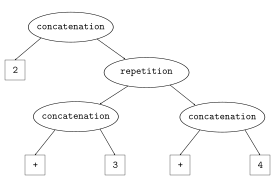
\includegraphics[width=0.5\textwidth]{ast}
		\caption{\emph{The Abstract Syntax Tree of the expression: 2 + 3 + 4}}
		\label{fig:ast}
\end{figure}

Naturally, the node representing a \texttt{repetition} may have an unlimited number of children while
\texttt{concatenation} always has two.

The data structure representing a node of the AST can be found inside the \texttt{base\_rule} class:
\begin{center}
	\begin{minipage}[h]{0.9\textwidth}
		\begin{lstlisting}[language=C++, breaklines=true, numbers=left]
struct node {
	enum class type {value, alternation, concatenation, option, repetition, repetition_or_epsilon, named_rule};

	type the_type;
	std::string the_value;
	std::vector<std::shared_ptr<node>> children;

	node(std::string a_value): the_type(type::value),the_value(a_value) {}

	node(type a_type): the_type(a_type) {}
};
		\end{lstlisting}
	\end{minipage}
\end{center}

The type of the node can determined using \texttt{the\_type} member which has one of the values of the
\texttt{type} enumeration. The nodes could be represented by a class hierarchy with one class assigned to each
operator, one to the named rules and one that would serve as a leaf node. This idea was rejected as the
typical use case of tree traversal will branch depending on the node type so in case of a class hierarchy a
complex \texttt{if} structure would appear with \texttt{dynamic\_cast}s which has a larger time cost then
switching based on an enumeration. In order to make use of polymorphism in case of a class hierarchy, the
visitor pattern could possibly be used but that would complicate an already complex, recursive tree traversal
algorithm.

The subtrings matched by the character-level rules are stored in \texttt{the\_value} member.

A node might have no children at all, or it might have an unlimited number of offsprings. They are stored in
the \texttt{children} container. Nodes are created dynamically and stored using \texttt{shared\_ptr}s. 

There is a type called \texttt{named\_rule} to support a feature that enables users to add extra nodes to an
AST corresponding to user defined non-terminals.  More about this can be found later.

If the AST is needed, the \texttt{base\_rule::set\_build\_ast(true);} call has to be issued before parsing
(line~2) and the reference of the root of the AST (line~13) to be built has to be given to the \texttt{match}
method call of the highest level rule (line~15) as seen below:

\begin{center}
	\begin{minipage}[h]{0.85\textwidth}
		\begin{lstlisting}[language=C++, breaklines=true, numbers=left]
int main() {
	base_rule::set_build_ast(true);

	rule addition, addend, expression;

	addition <<= -addend << *(-character("+") << -addend);
	addend <<= -range('0', '9') | -expression;
	expression <<= -character("(") << -addition << -character(")");

	std::string input = "2 + 3 + 4\n";
	base_rule::match_range context(input.cbegin(), input.cend());
	base_rule::match_range result;
	std::shared_ptr<base_rule::node> root;

	if (addition.match(context, result, root)) {
		std::cout << "Matched: " << std::string(result.first, result.second);
		parse_tree(root);
	} else {
		std::cout << "Didn't match";
	}
}
		\end{lstlisting}
	\end{minipage}
\end{center}

This example also shows how the whitespaces can be consumed using the operators \texttt{-} or \texttt{$\sim$}.

The resulting AST can be traversed by writing a simple recursive function such as the one in the following
example. Line~17 in the code above shows how it should be called.

\begin{center}
	\begin{minipage}[h]{0.95\textwidth}
		\begin{lstlisting}[language=C++, breaklines=true, numbers=left]
void parse_tree(std::shared_ptr<base_rule::node> const &node, size_t depth=0) {
	if (node) {
		for (size_t i = 0; i < depth; ++i) std::cout << " ";

		switch (node->the_type) {
			case base_rule::node::type::value:
				std::cout << node->the_value << std::endl;
			break;

			case base_rule::node::type::alternation:
				std::cout << "alternation" << std::endl;
			break;

			case base_rule::node::type::concatenation:
				std::cout << "concatenation" << std::endl;
			break;

			case base_rule::node::type::option:
				std::cout << "option" << std::endl;
			break;

			case base_rule::node::type::repetition:
				std::cout << "repetition" << std::endl;
			break;

			case base_rule::node::type::repetition_or_epsilon:
				std::cout << "repetition_or_epsilon" << std::endl;
			break;

			case base_rule::node::type::named_rule:
				std::cout << "named_rule: " << node->the_value << std::endl;
			break;
		}

		for (auto &a_node: node->children) parse_tree(a_node, depth + 1);
	}
}
		\end{lstlisting}
	\end{minipage}
\end{center}

The \texttt{named\_rule} type is special and is discussed later.

Earlier we have discussed the code of \texttt{match} and \texttt{test} methods. Those listings were not
identical to the actual code of these methods found in the framework as the parts concering the building of
the AST were omitted.

Actually only a little needs to be added to those methods. Both of them receive an extra argument: the
reference of a pointer to the subtree's root that has to be built by the rule. This pointer is overwritten
with the address of the newly created node and the tree is created by the successive recursive function calls
as the parser digs into the text. The default value of this argument is the reference of a static node -- this
is needed as a reference has to be initialized, but it would be cumbersome for the user to give a root
reference even if an AST is not needed\footnote{The \texttt{match} method could have been overloaded, but the
code of the two function would have been almost identical, so that was considered as bad style.}.

The method \texttt{match} simply delegates the given pointer to the \texttt{test} function.

The \texttt{test} method of character-level rules and high-level rules are different so an example for both
are discussed below.

First, let's dwelve into the code of \texttt{character} class's \texttt{test} method. This is a class that
operates at the character-level so it has to produce a leaf node in the AST, one that has no children and
contains the result of a match (a string containing a single character in this case).

The only difference to the code seen earlier apart from the extra argument is that it creates a new node in
line~14 and saves its address in the \texttt{ast\_root} variable. This is only done if an AST is needed,
otherwise time and memory is not wasted on it.

The \texttt{get\_build\_ast()} call reads the value of the static \texttt{build\_ast} variable.

The value of the node is set by creating a \texttt{std::string} object using the \texttt{const\_iterator}s
of \texttt{the\_match\_range}. No children are set which results in two null pointers showing that this node
is a leaf.

\begin{center}
	\begin{minipage}[ht]{0.95\textwidth}
		\begin{lstlisting}[language=C++, breaklines=true, numbers=left]
bool character::test(base_rule::match_range &context, match_range &the_match_range, std::shared_ptr<base_rule::node> &ast_root) {
	if (context.first == context.second) return false;

	base_rule::match_range local_context = context;

	for (auto allowed_character: allowed_characters) {
		if (*local_context.first == allowed_character) {
			++local_context.first;

			the_match_range.first = context.first;
			the_match_range.second = local_context.first;
			context = local_context;

			if (get_build_ast()) ast_root = std::make_shared<base_rule::node>(std::string(the_match_range.first, the_match_range.second)); 

			return true;
		}
	}

	return false;
}
		\end{lstlisting}
	\end{minipage}
\end{center}

The other type of \texttt{test} method can be found in the high-level rules that are instantiated using
operators. The code below belongs to the \texttt{concatenation} rule.

\begin{center}
	\begin{minipage}[ht]{0.95\textwidth}
		\begin{lstlisting}[language=C++, breaklines=true, numbers=left]
bool concatenation::test(base_rule::match_range &context, base_rule::match_range &the_match_range, std::shared_ptr<base_rule::node> &ast_root) {
	base_rule::match_range first_range, second_range;
	base_rule::match_range local_context = context;
	std::shared_ptr<base_rule::node> first_child, second_child;

	if (first->match(local_context, first_range, first_child) && second->match(local_context, second_range, second_child)) {
		the_match_range.first = first_range.first;
		the_match_range.second = second_range.second;
		context = local_context;

		if (get_build_ast()) {
			ast_root = std::make_shared<base_rule::node>(base_rule::node::type::concatenation);
			ast_root->children.push_back(first_child);
			ast_root->children.push_back(second_child);
		}

		return true;
	}
	else return false;
}
		\end{lstlisting}
	\end{minipage}
\end{center}

This rule creates a node that always has two children: one for each of the two rules following eachother. The
rule calls two rules that have to match for this one to be successful. Those rules can be very complex and
create a large subtree each.

The roots of the two subtrees are created locally in line~4 and fed to the two subrules in line~6. If the
match is successful and an AST is needed then a new node is created in line~12. This one is not constructed
with the string containing the match range as it could be a complex match of several rules and would be of
little use to the user. This node will tell the traversing algorithm the type of operator that matched at the
current position instead. It is \texttt{type::concatenation} in this case.

The children of this node are the two nodes (or subtrees) that are created by the \texttt{match} calls of the
inner rules of \texttt{concatenation} in line~6. They are added to the node in the lines~13 and 14.

Finally the code of \texttt{repetition::test} is also listed here to show how an unlimited number of children
can be handled.

\begin{center}
	\begin{minipage}[ht]{0.95\textwidth}
		\begin{lstlisting}[language=C++, breaklines=true, numbers=left]
bool repetition::test(base_rule::match_range &context, base_rule::match_range &the_match_range, std::shared_ptr<base_rule::node> &ast_root) {
	base_rule::match_range range;
	base_rule::match_range local_context = context;
	std::shared_ptr<base_rule::node> child;

	if (repeated_rule->match(local_context, range, child)) {
		the_match_range = range;

		if (get_build_ast()) {
			ast_root=std::make_shared<base_rule::node>(base_rule::node::type::repetition);
			ast_root->children.push_back(child);
		}

		while (repeated_rule->match(local_context, range, child)) {
			the_match_range.second = range.second;

			if (get_build_ast()) {
				ast_root->children.push_back(child);
			}
		}

		context = local_context;

		return true;
	}

	return false;
}
		\end{lstlisting}
	\end{minipage}
\end{center}

It is important to note that the node is created only once (when the first child is added). When the
\texttt{while} loop is entered in line~14, the node already exists, so a child can be added to it in line~18.
This situation is handled similarly in \texttt{repetition\_or\_epsilon::test}, the code of which is not listed
here. The reader is encouraged to have a look at it though.

There is one additional feature of SyntX's AST-building facilities that's worth mentioning. At the beginning
of this subsection it was stated that ASTs represent the grammatical structure of the text and not the
internal logic of the text. Fortunately this is not entirely true: the users of the framework can add extra
nodes to the tree representing their rules. In order to do that, a rule created by the user has to be supplied
with a name at construction.

So let's change our little example as follows.

\begin{center}
	\begin{minipage}[ht]{0.85\textwidth}
		\begin{lstlisting}[language=C++, breaklines=true, numbers=left]
int main() {
	base_rule::set_build_ast(true);

	rule addition, addend("addend"), expression;

	addition <<= -addend << *(-character("+") << -addend);
	addend <<= -range('0', '9') | -expression;
	expression <<= -character("(") << -addition << -character(")");

	std::string input = "2 + 3 + 4\n";
	base_rule::match_range context(input.cbegin(), input.cend());
	base_rule::match_range result;
	std::shared_ptr<base_rule::node> root;

	if (addition.match(context, result, root)) {
		std::cout << "Matched: " << std::string(result.first, result.second);
		parse_tree(root);
	} else {
		std::cout << "Didn't match";
	}
}
		\end{lstlisting}
	\end{minipage}
\end{center}

The only difference to the previously seen version is that the rule \texttt{addend} was given a name in
line~4.

The AST generated will now look like this:

\begin{figure}[h!]
	\centering
		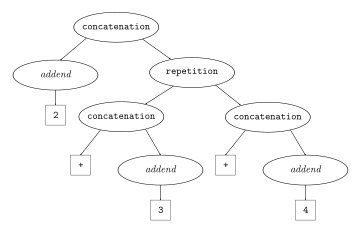
\includegraphics[width=0.7\textwidth]{ast_named_rule}
		\caption{\emph{The Abstract Syntax Tree of an expression with a named rule (addend)}}
		\label{fig:ast}
\end{figure}

This might not seem very useful in this rather simple example but it becomes very handy when a huge AST based
on a complex grammar has to be processed.

All it took to achieve this feature was to give the class \texttt{rule} a new member (\texttt{rule\_name}),
a new constructor that actually sets this name and the \texttt{test} function had to be altered a bit.

\begin{center}
	\begin{minipage}[ht]{0.9\textwidth}
		\begin{lstlisting}[language=C++, breaklines=true, numbers=left]
bool rule::test(match_range &context, match_range &the_match_range, std::shared_ptr<base_rule::node> &ast_root) {
	if (!(*the_rule)) throw undefined_rule();
	if (!get_build_ast() || rule_name == "")
		return (*the_rule)->match(context, the_match_range, ast_root);
	else {
		std::shared_ptr<base_rule::node> child;
		if ((*the_rule)->match(context, the_match_range, child)) {
			if (child) {
				ast_root = std::make_shared<base_rule::node>(base_rule::node::type::named_rule);
				ast_root->the_value = rule_name;
				ast_root->children.push_back(child);
			}
			return true;
		}
		else return false;
	}
}
		\end{lstlisting}
	\end{minipage}
\end{center}

If the rule doesn't have a name (i.e. the \texttt{rule\_name} member is an empty string) or the AST was not
requested by the user then the \texttt{test} method merely delegates the context, the match range and root of
the AST to the inner \texttt{base\_rule} that is wrapped by it. This can be seen in lines~3 and 4. 

On the other hand, if the rule has a name and we are building an AST, an extra node has to be inserted. In
order to do this, a child node is created and fed to the inner rule (lines~6 and 7) and then a new node is
created in line~9. It is of type \texttt{named\_rule} and its name is stored in \texttt{the\_value} member of
the node (line~10).

The child that is created by the inner rule is set as the child of the named rule node in line~11.

All this happens only if a child is indeed created by the inner rule. If the inner rule is an \texttt{option}
or a \texttt{repetition\_or\_epsilon} then it may match successfully an empty string. In this case these rules
will add null pointer to the tree to show that there is where the tree ends in the current direction. This
case can be easily checked by converting the child pointer to a boolean value and checking whether it is true
-- this happens in line~8.

If this check was omitted, a \texttt{named\_rule} node would be inserted in the tree without children which
could mislead the processing algorithm or simply make it necessary to add an extra conditional statement
testing whether a named rule is really there. This would be very cumbersome.

\vfill
\vfill
\vfill
\hfill\begin{minipage}[h]{0.3\textwidth}
\begin{center}
	\textit{Gergely Nagy}\\
	\textit{Budapest, \today}
\end{center}
\end{minipage}
\vfill

\newpage \tableofcontents

\vfill
\vfill
\begin{center}
\footnotesize\emph{Please consider the environment before printing this document.}
\end{center}
\vfill
\end{document}
